\documentclass{beamer}
\usetheme{Berkeley}
\usepackage{graphics}
\usepackage{fancybox}
%\usepackage{beamerthemesplit}


\title{Team PICA}
\subtitle{\textbf{P}ower \textbf{I}nformation \textbf{C}ollection \textbf{A}rchitecture}
\author{Kendrick Wiersma}
\institute{Calvin College Engineering Department}
%\institute{
\includegraphics[height=.35in]{includes/calvin_minds}}
\date{15 April 2011}

\begin{document}
\logo{
\includegraphics[scale=.5]{includes/calvin_minds.png}}
\begin{frame}
\titlepage
\vspace{-0.4in}
\begin{center}

\includegraphics[height=1in]{includes/pica_logo}
\end{center}
\end{frame}
%----------- Outline --------------------%
\section[Outline]{}
\begin{frame}
\tableofcontents
\end{frame}
%----------- Team Introduction --------------------%
\section{Team Introduction}
\begin{frame}\frametitle{Team Introduction}
\begin{figure}[htbp]
\begin{center}
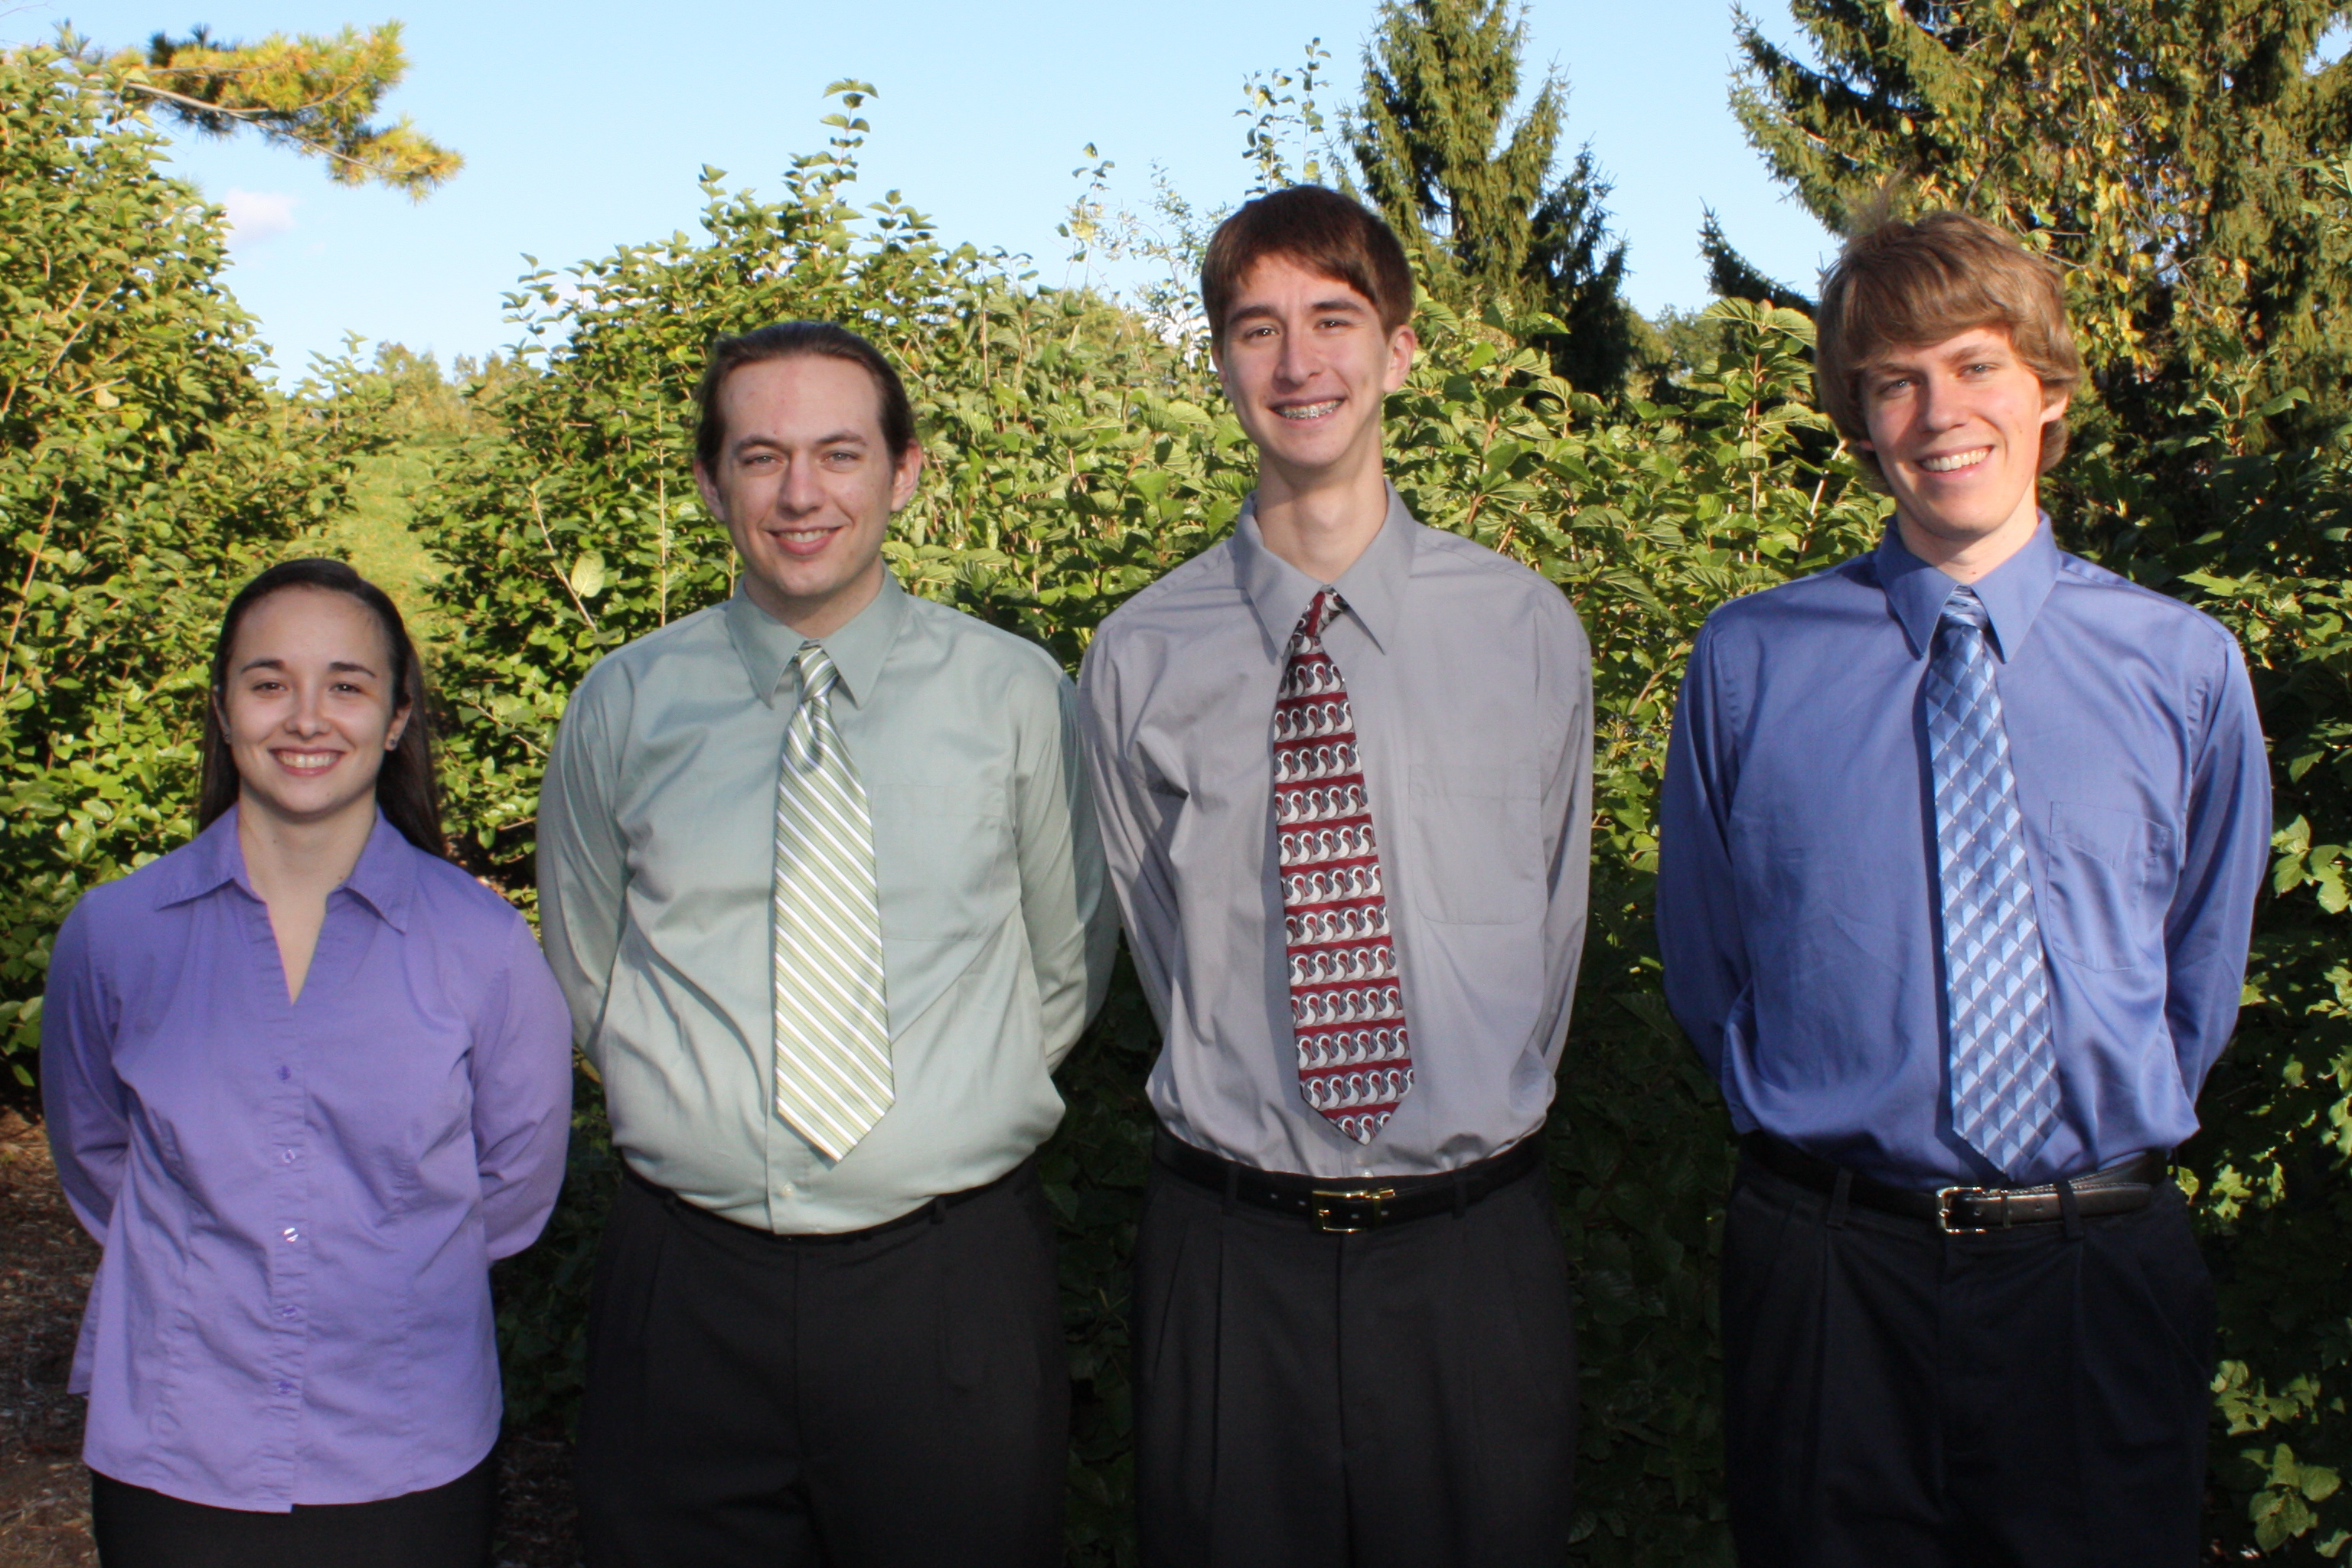
\includegraphics[width=3.5in]{includes/IMG_0865}
\caption{Amy Ball (EE), Kendrick Wiersma (EE), Nate Jen (EE), Avery Sterk (EE)}
\label{fig:team_pic}
\end{center}
\end{figure}
\end{frame}


\section{Project Introduction}
%\subsection{Problem Statement}
% -- Problem Statement Text Slide
\begin{frame}{Problem Statement and Project Goal}
\begin{block}{Problem Statement}
Traditional power metering devices provide a consumer with a single measurement over a long period of time. This situation does not allow consumers to actively monitor their own power usage making it more difficult to proactively conserve power.
\end{block}\pause
\begin{block}{Project Goal}
Provide instantaneous information about a consumer's power consumption to both the consumer and the power company in such a way that the data has meaning to each. Thus enabling the consumer to take a more proactive approach to conserving power.
\end{block}
\end{frame}

% -- Problem Statement Graphics Slide (Funny)
\begin{frame}
	\begin{columns}[t]
		\column{.5\textwidth}
			\begin{block}{From this...}
			\begin{center}
			
\includegraphics[scale=.3]{includes/high-utility-bill-shock}
			\end{center}
			\end{block}\pause
		\column{.5\textwidth}
			\begin{block}{To This...}
			\begin{center}
			
\includegraphics[height=2in]{includes/happyGirl}
			\end{center}
			\end{block}
		\end{columns}
\end{frame}

% -- Smart Metering Slide
%\subsection{Smart Metering}
\begin{frame}{Smart Metering}
	\begin{figure}
	\begin{center}
	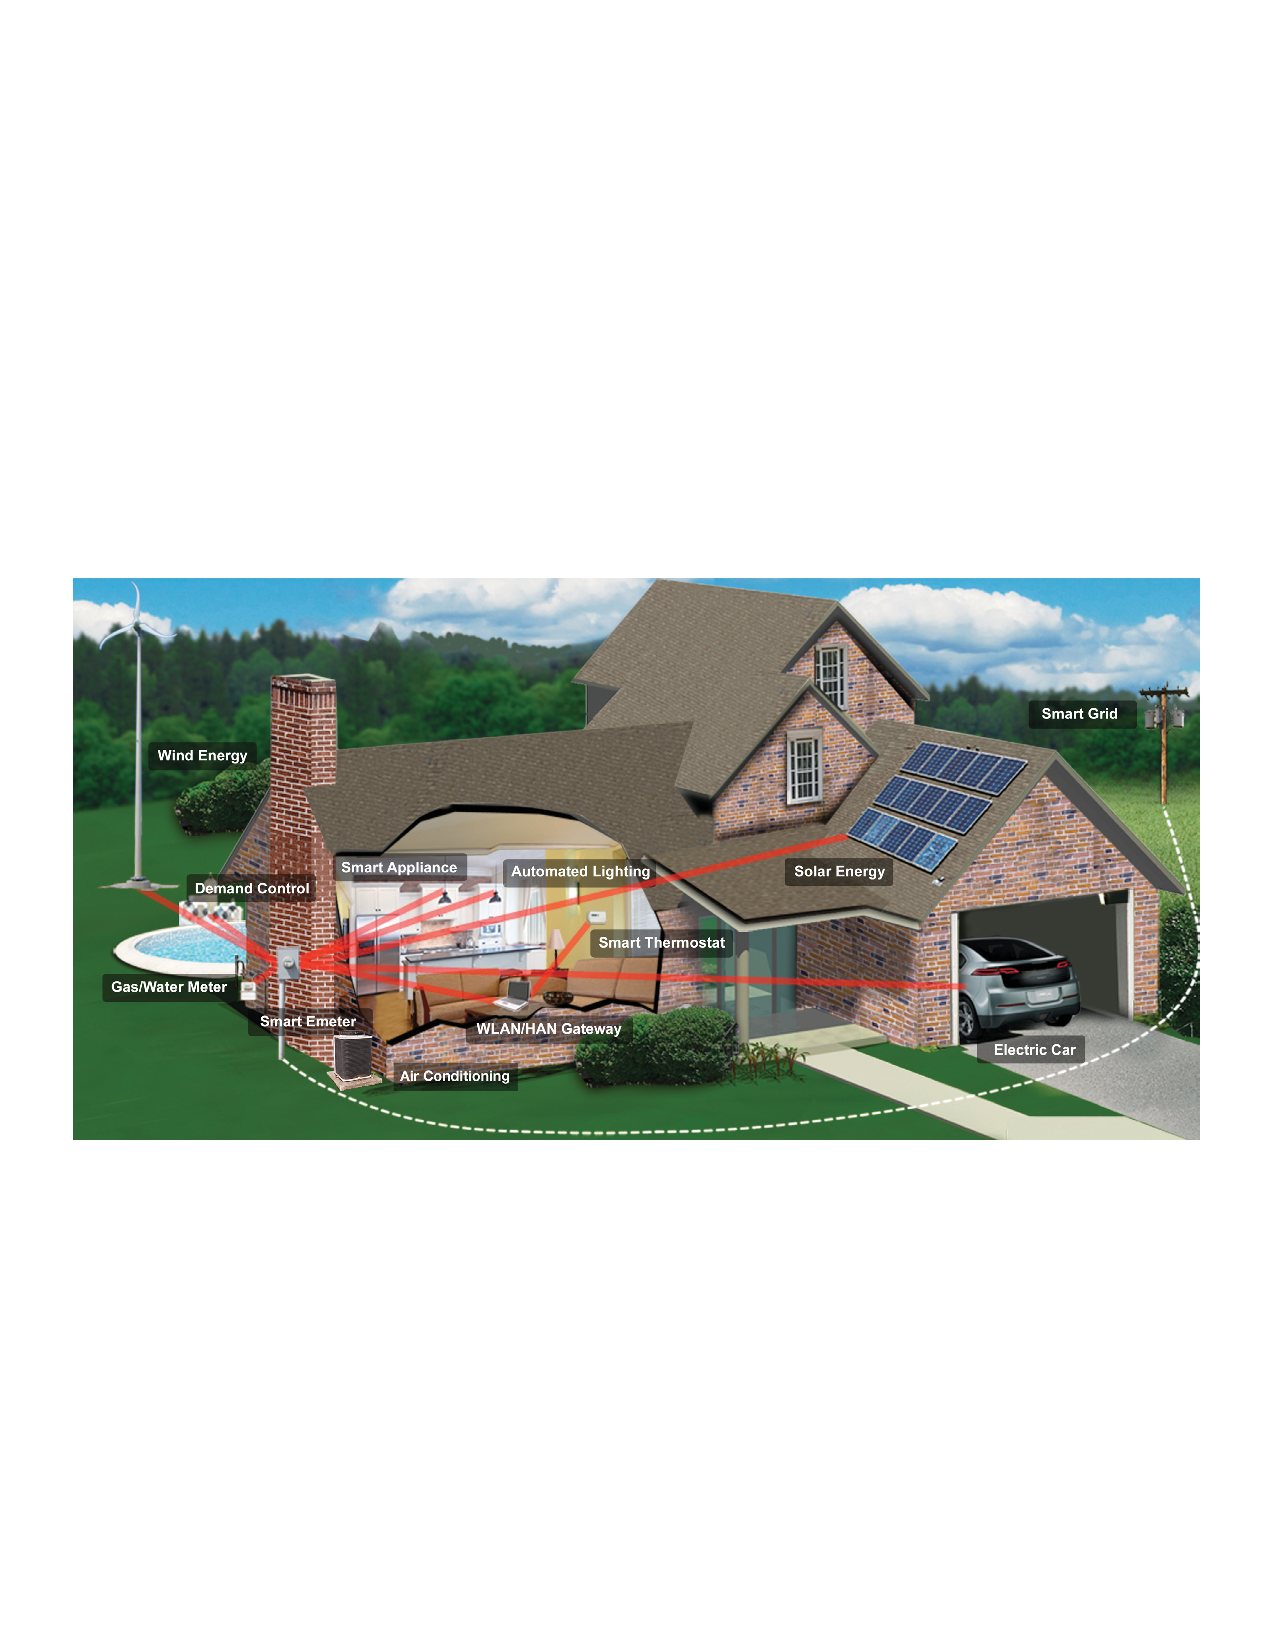
\includegraphics[width=4in]{includes/TI_smart_meter_picture}
	\caption{Smart metering diagram. {\footnotesize(Image copyright Texas Instruments.)}}
	\label{fig:smart_metering}
	\end{center}
	\end{figure}
\end{frame}

% -- What do we mean by smart meter
\begin{frame}{AMR vs. AMI}
	\begin{columns}[t]
		\column{.5\textwidth}
			\begin{block}{\footnotesize{Automated Meter Reading (AMR)}}
				{\footnotesize Provides one-way communication from the meter to the utility company. Removes the need for an employee to visit the meter each month and manually collect readings. AMR systems are not considered smart meters.}
			\end{block}\pause
		\column{.5\textwidth}
			\begin{block}{\footnotesize{Advanced Metering Infrastructure (AMI)}}
				{\footnotesize Provide two-way communication with the utility company and other nearby meters (such as gas, water, heat, etc. Allows for collection and distribution of data to and from the customer. Allows the supply system (electric grid) to respond to changes in demand.}
			\end{block}\pause
	\end{columns}
	\begin{alertblock}{Our Choice}
		Team PICA chose to implement an Advanced Metering Infrastructure System.
	\end{alertblock}
\end{frame}

%\subsection{Our Project}
% -- Discussion of our subsystems
\begin{frame}{The PICA System}

\centering{\ovalbox{\Large The Three PICA Subsystems}}\pause
\begin{columns}[t]
	\column{.3\textwidth}
		\begin{center}
		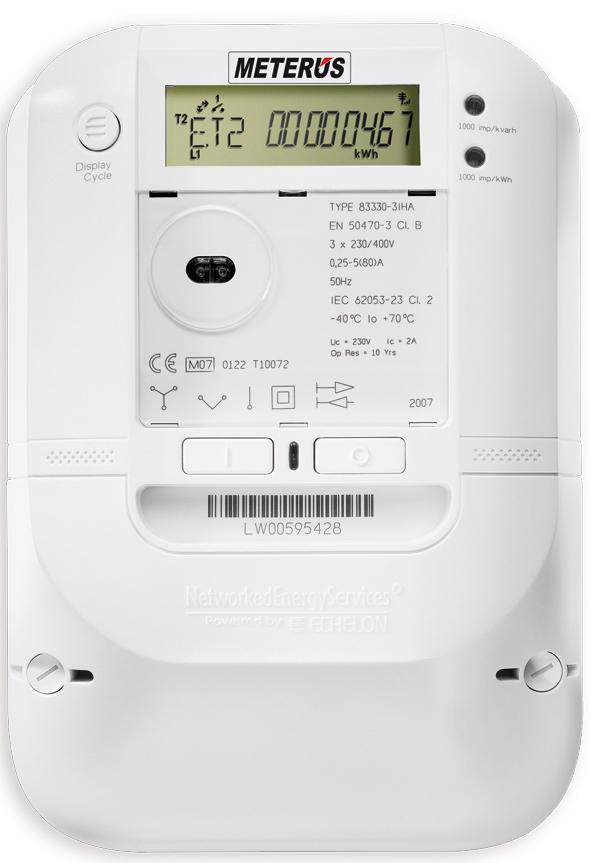
\includegraphics[height=1in]{includes/europe_smart_meter}\\
		\shadowbox{E-Meter}
		\end{center}\pause
	\column{.3\textwidth}
		\begin{center}
		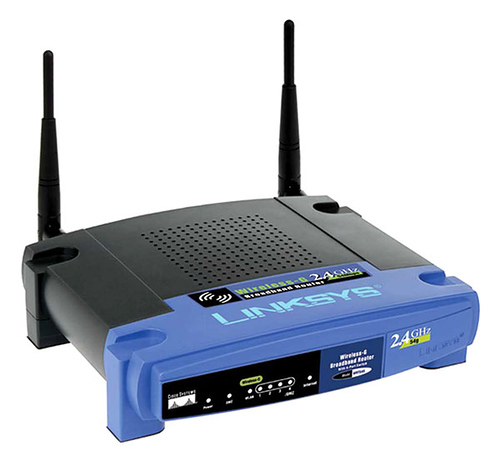
\includegraphics[width=1in]{includes/wrt54g}\\
		\shadowbox{Base Station}
		\end{center}\pause
	\column{.3\textwidth}
		\begin{center}
		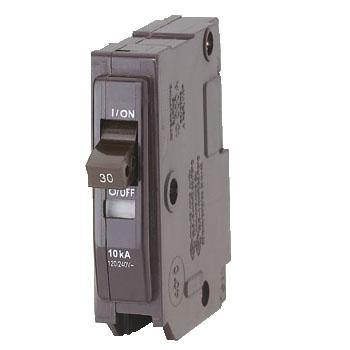
\includegraphics[width=1in]{includes/reset-circuit-breaker}\\
		\shadowbox{Smart Breakers}
		\end{center}
\end{columns}
\end{frame}

\section{E-Meter}
%\subsection{Purpose}
% -- Intro to the E-Meter
\begin{frame}{E-Meter}
	\begin{block}{Purpose}
		\begin{itemize}
		\item <1-> Accumulate kilowatt-hours of energy used
		\item <2-> Monitor voltage (1-3 phase)
		\item <3-> Monitor current flow (1-3 phase)
		\item <4-> Display data on integrated LCD screen
		\item <5-> Transmit data to consumer and utility company
		\end{itemize}
	\end{block}
\end{frame}
%\subsection{Hardware Design}

% -- E-Meter Hardware design
\begin{frame}{E-Meter Hardware}
	\begin{figure}[htbp]
	\begin{center}
	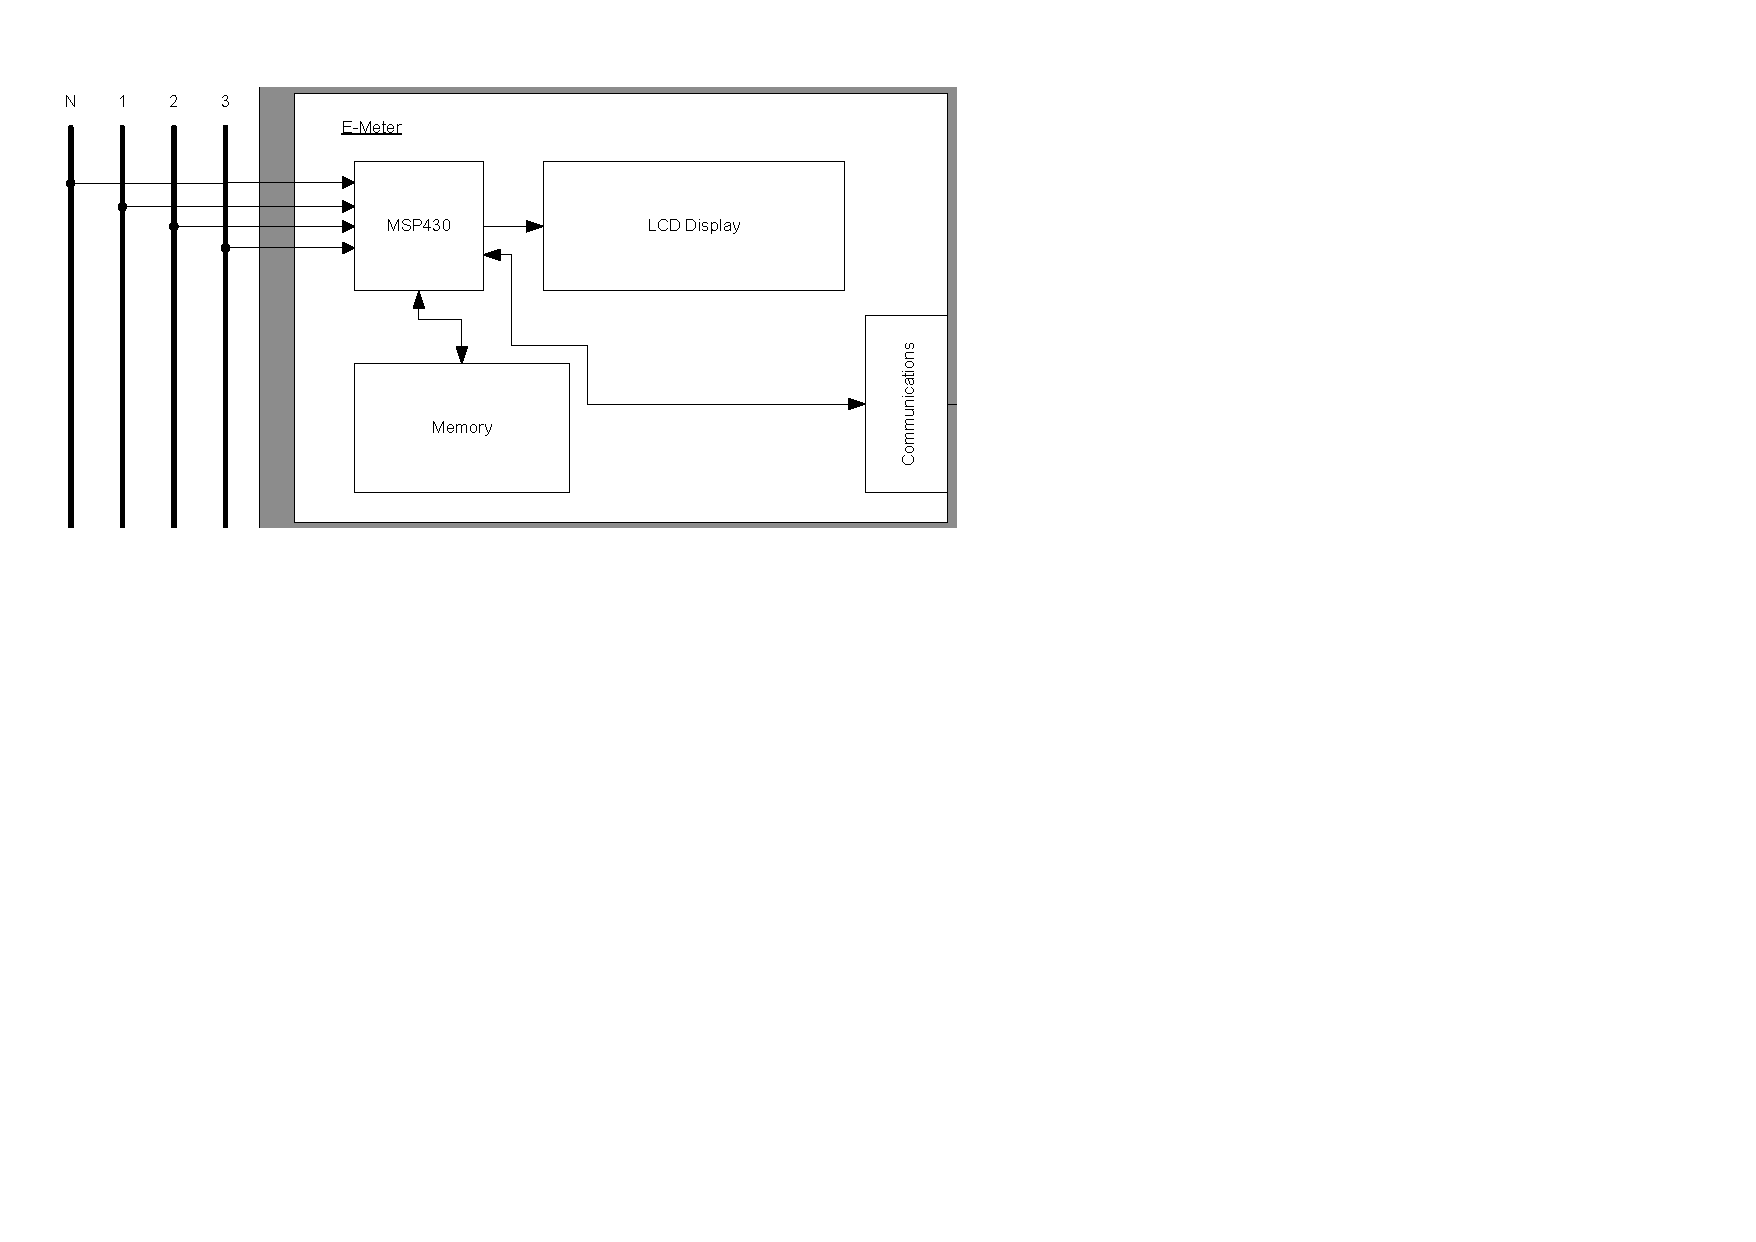
\includegraphics[width=4in]{includes/e_meter_diagram}
	\caption{E-Meter hardware diagram.}
	\label{fig:e_meter_diagram}
	\end{center}
	\end{figure}
\end{frame}
\begin{frame}{E-Meter Hardware}
	\begin{itemize}
		\item <1 -> Centered on TI MSP430F47197
		\item <2 -> Uses 3 current transformers, 1 for each phase attached to MSP430 ADC
		\item <3 -> Uses 3 voltage shunts, 1 for each phase attached to MSP430 ADC
		\item <4 -> SynchroSystems 160-segment 4-mux LCD on the MSP430 internal LCD driver
		\item <5 -> MAX233A RS232 serial driver for serial communications
		\item <6 -> Xbee wireless communications device
	\end{itemize}
\end{frame}

%\subsection{Software Design}
\begin{frame}{E-Meter Software}
	\begin{figure}[htbp]
	\begin{center}
	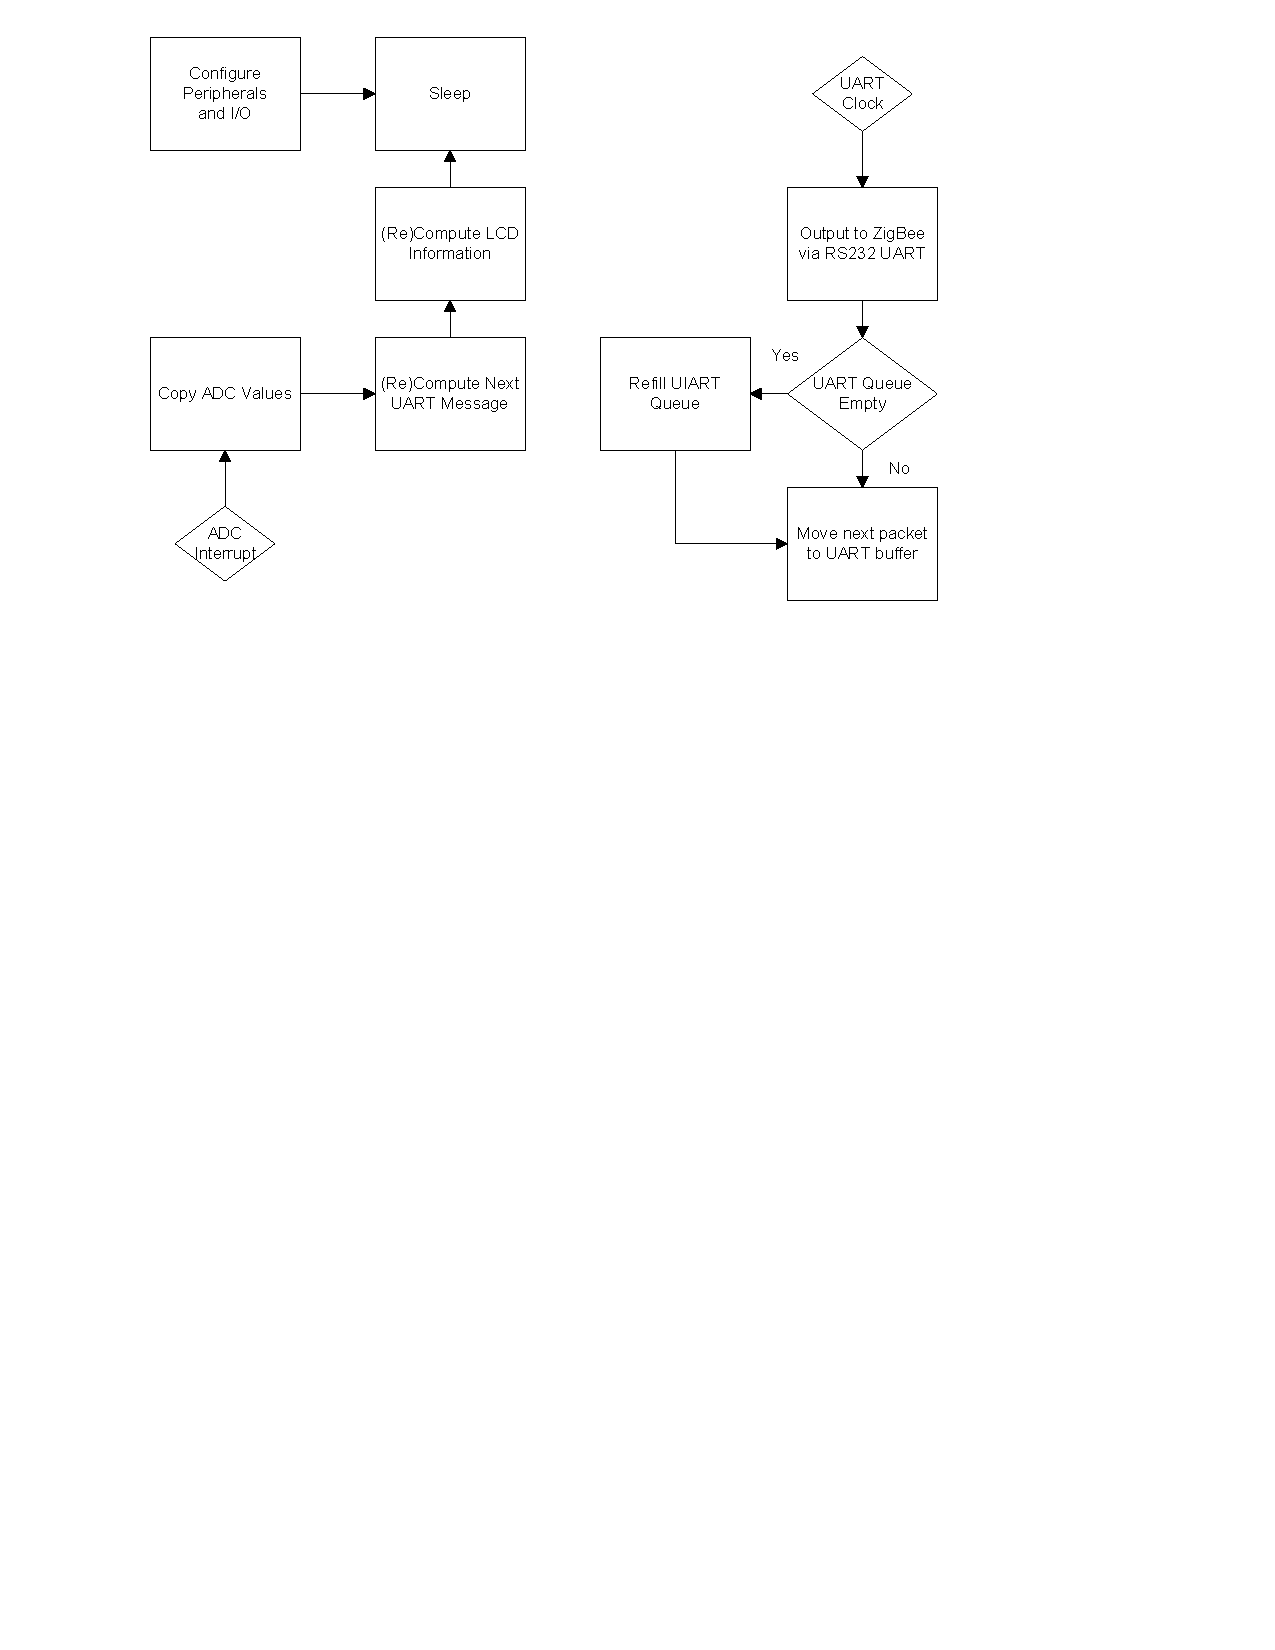
\includegraphics[width=3.5in]{includes/E_Meter_Software_Flowchart}
	\caption{E-Meter Software Flowchart}
	\label{fig:e_meter_software_flow}
	\end{center}
	\end{figure}
\end{frame}

\section{Base Station}
%\subsection{Purpose}
\begin{frame}{Base Station}
	\begin{block}{Purpose}
		\begin{itemize}
		\item <1 -> Aggregate data from other systems and process for display to user
		\item <2 -> Host webpage interface to the PICA system
		\item <3 -> Control Xbee network
		\end{itemize}
	\end{block}
\end{frame}

%\subsection{Hardware Design}
\begin{frame}{Base-Station Hardware}
	\begin{figure}[htbp]
	\begin{center}
	\fbox{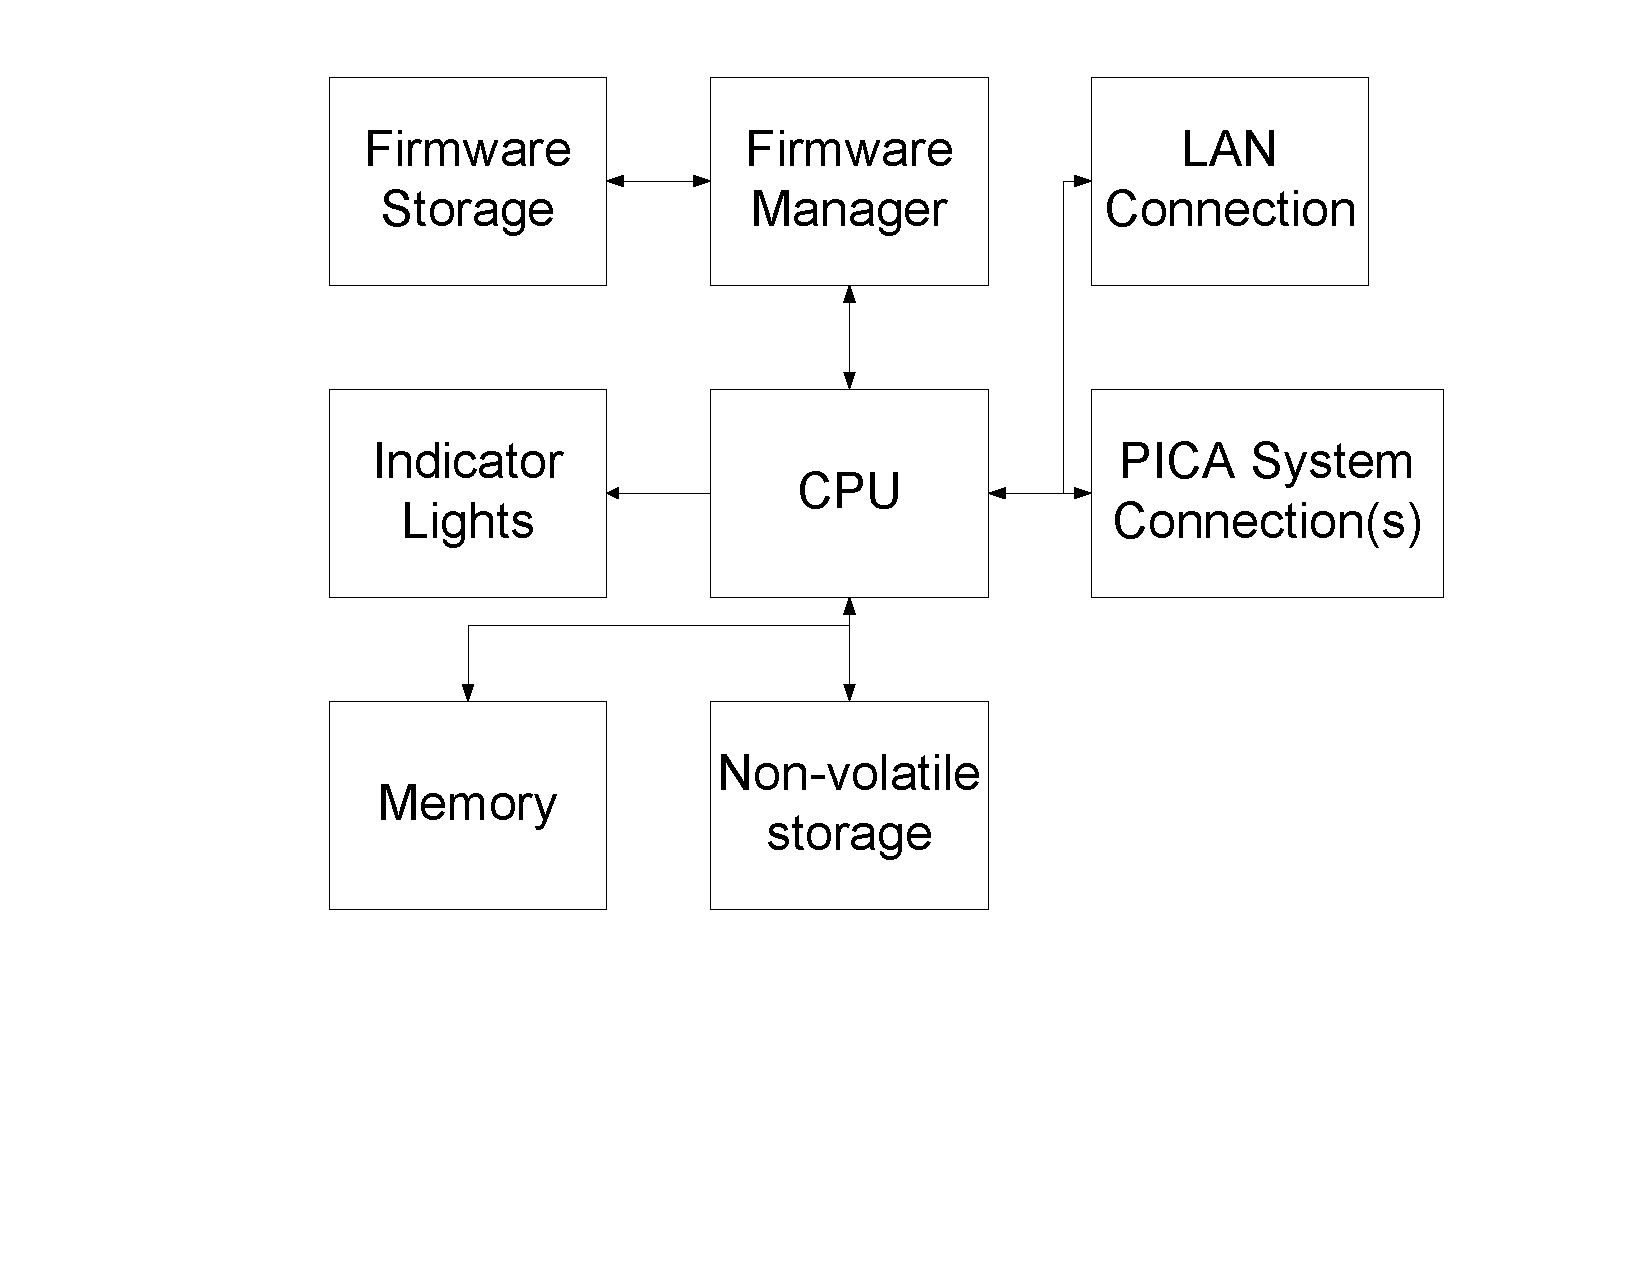
\includegraphics[width=3in]{includes/Base_Station_Block_Diagram}}
	\caption{Base station hardware block diagram.}
	\label{fig:base_station_blocks}
	\end{center}
	\end{figure}
\end{frame}

\begin{frame}{Base-Station Hardware (continued)}
	\begin{itemize}
		\item <1 -> Centered on synthesizable LEON3 SPARC V8 from Gaisler Aerospace (GPL)
		\item <2 -> Built on Digilent ML-509 Xilinx Virtex 5 development board
		\item <3 -> Serial connection to Xbee collector
	\end{itemize}
\end{frame}

\begin{frame}{Base-Station Software}
	\begin{itemize}
		\item <1 -> Run a custom compiled Linux kernel based on 2.6.35 (GNU)
		\item <2 -> Use Apache as a webserver (Apache License)
		\item <3 -> Build a custom app to read data from the serial port, process the incoming data and format it for webpage.
	\end{itemize}
\end{frame}

\begin{frame}{Base-Station Dropped}
	\begin{alertblock}{Project Component Dropped}
		Due to time constraints on the design team, a separate hardware base-station has been dropped from the project. As a replacement, the team will design the software to run on a standard x86 Linux PC.
	\end{alertblock}
\end{frame}

% -- Smart Breakers
\section{Smart Breakers}
\begin{frame}{Solid State Breakers}
	\begin{figure}[htbp]
	\begin{center}
	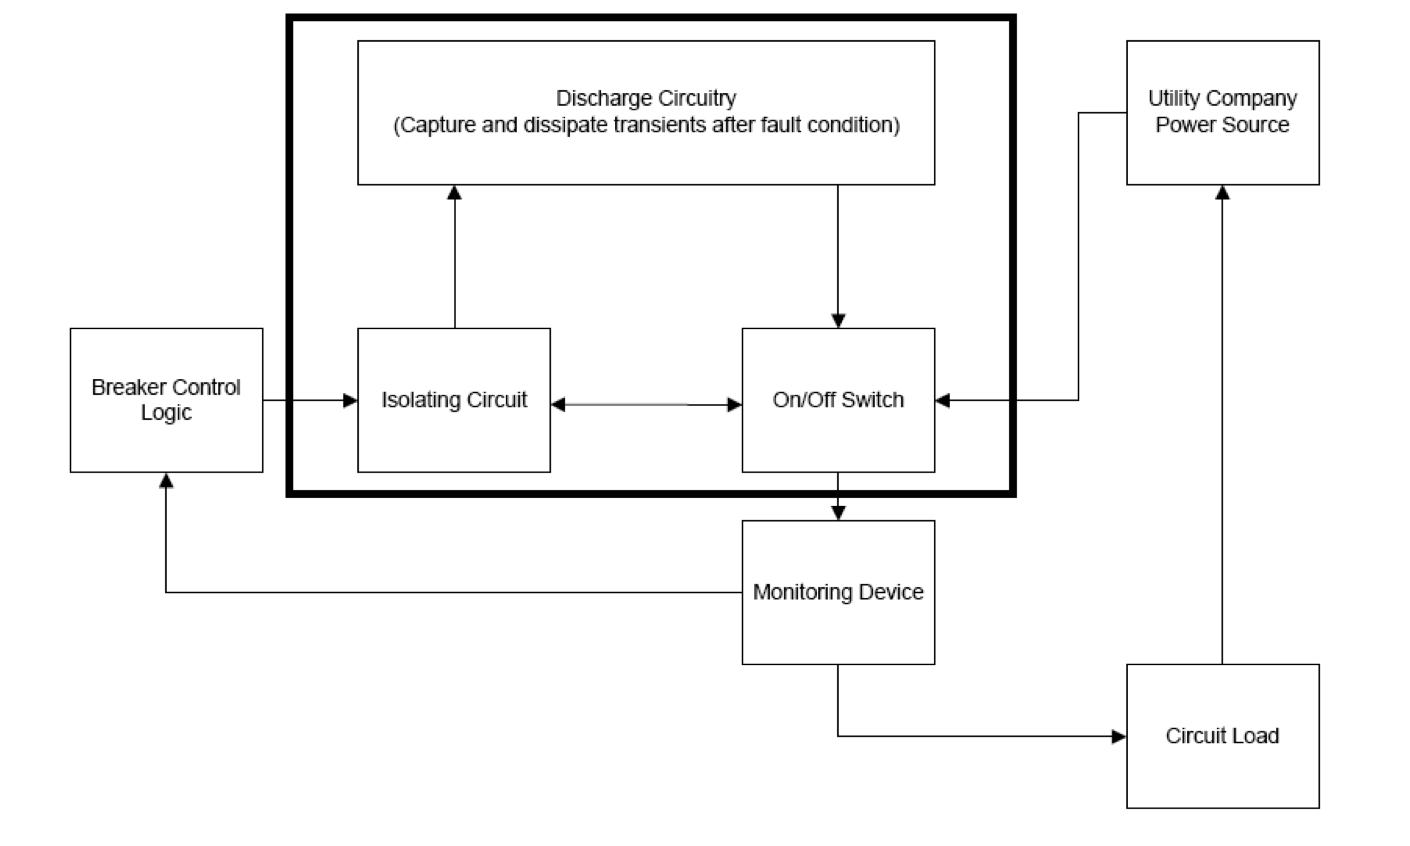
\includegraphics[width=4in]{includes/SSB_Functional_Diagram}
	\caption{Block diagram of the smart breakers.}
	\label{fig:ssb_block_diagram}
	\end{center}
	\end{figure}
\end{frame}

\begin{frame}{Smart Breakers (Continued)}
	\begin{block}{Purpose}
		\begin{itemize}
		\item <1-> Replace a traditional air-gap circuit interruptor with solid-state components
		\item <2 -> Monitor current passing though solid-state interruptor
		\item <3 -> Automatic detection of over-current situation
		\item <4 -> Automatic detection of over-voltage situation
		\end{itemize}
	\end{block}
\end{frame}

\begin{frame}{Smart Breakers Hardware}
	\begin{figure}[htbp]
	\begin{center}
	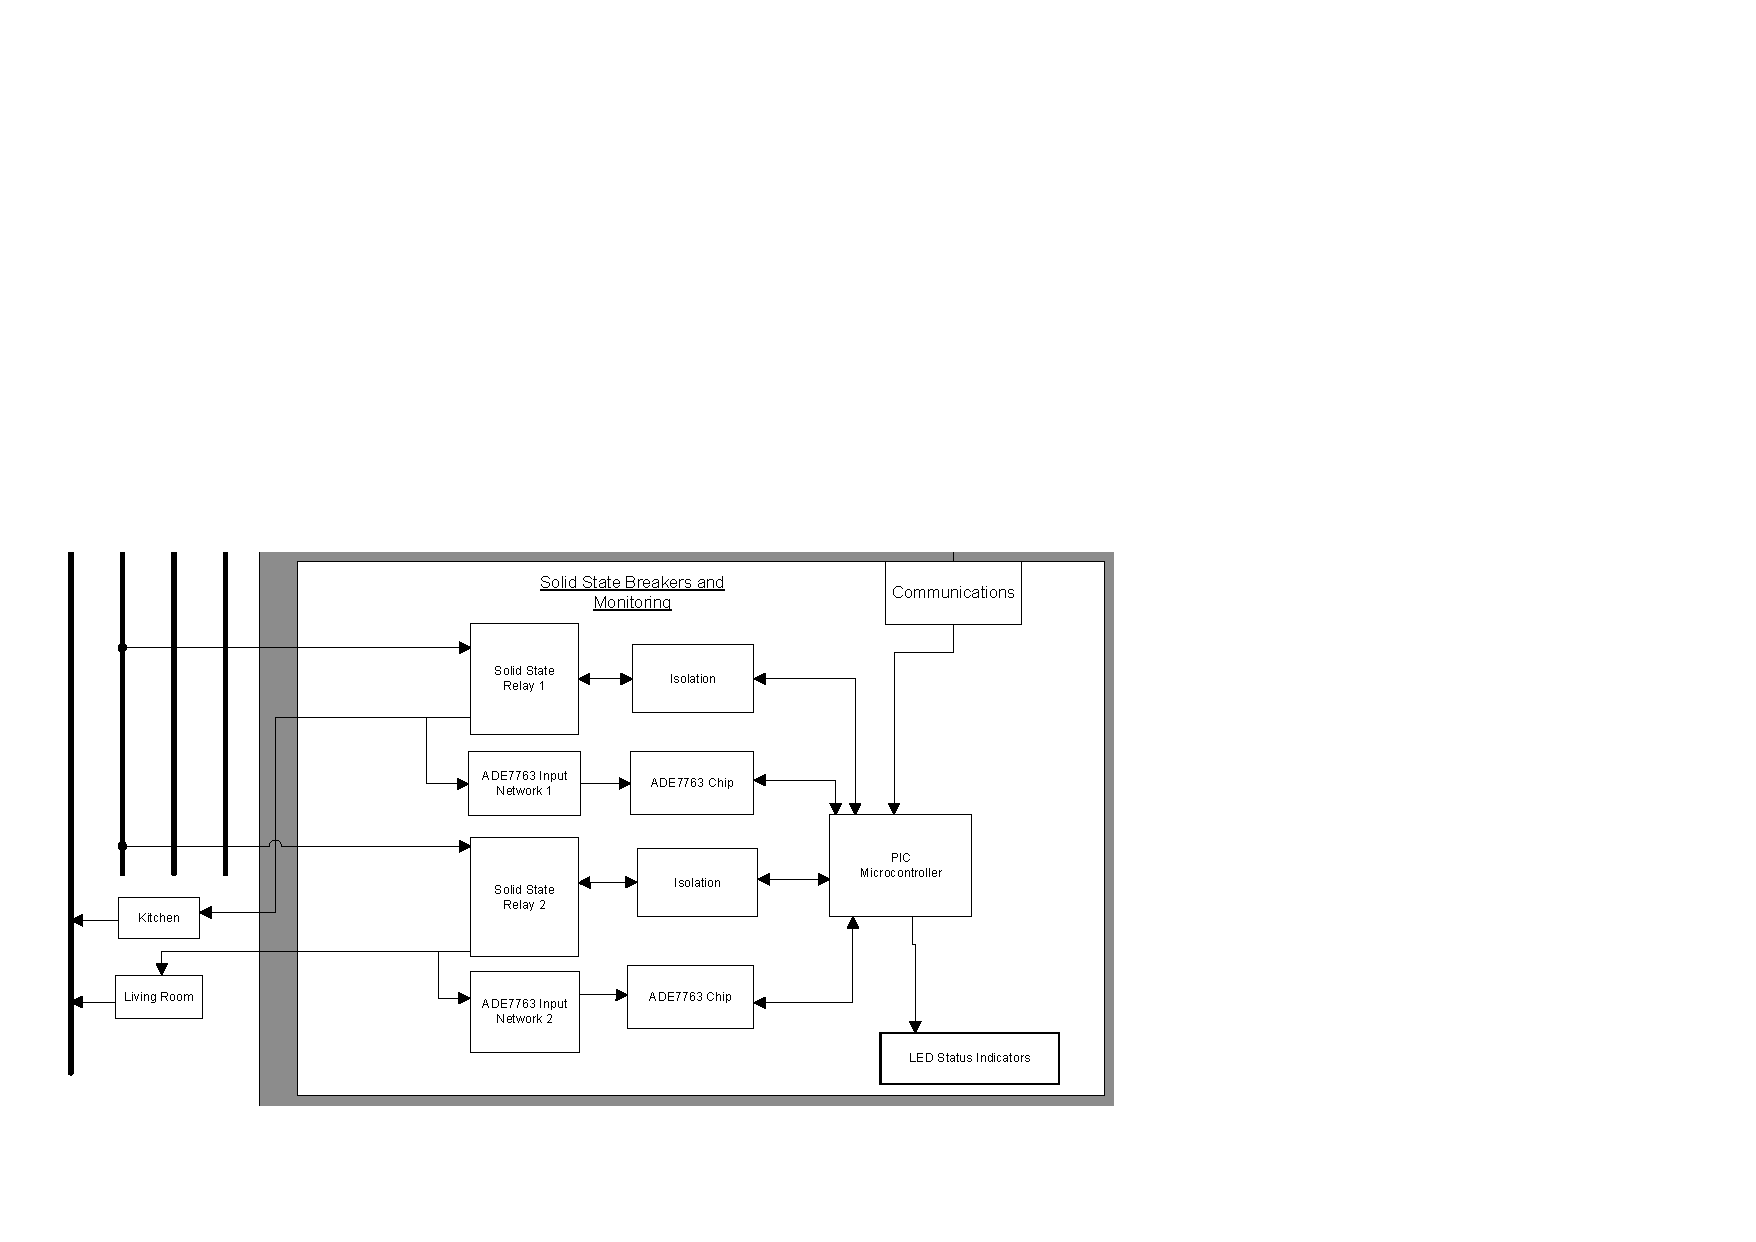
\includegraphics[width=4in]{includes/smart_breaker_diagram}
	\caption{Smart breakers hardware diagram.}
	\label{fig:smart_break_diagram}
	\end{center}
	\end{figure}
\end{frame}

\begin{frame}{Smart Breakers Software}
	\begin{figure}[htbp]
	\begin{center}
	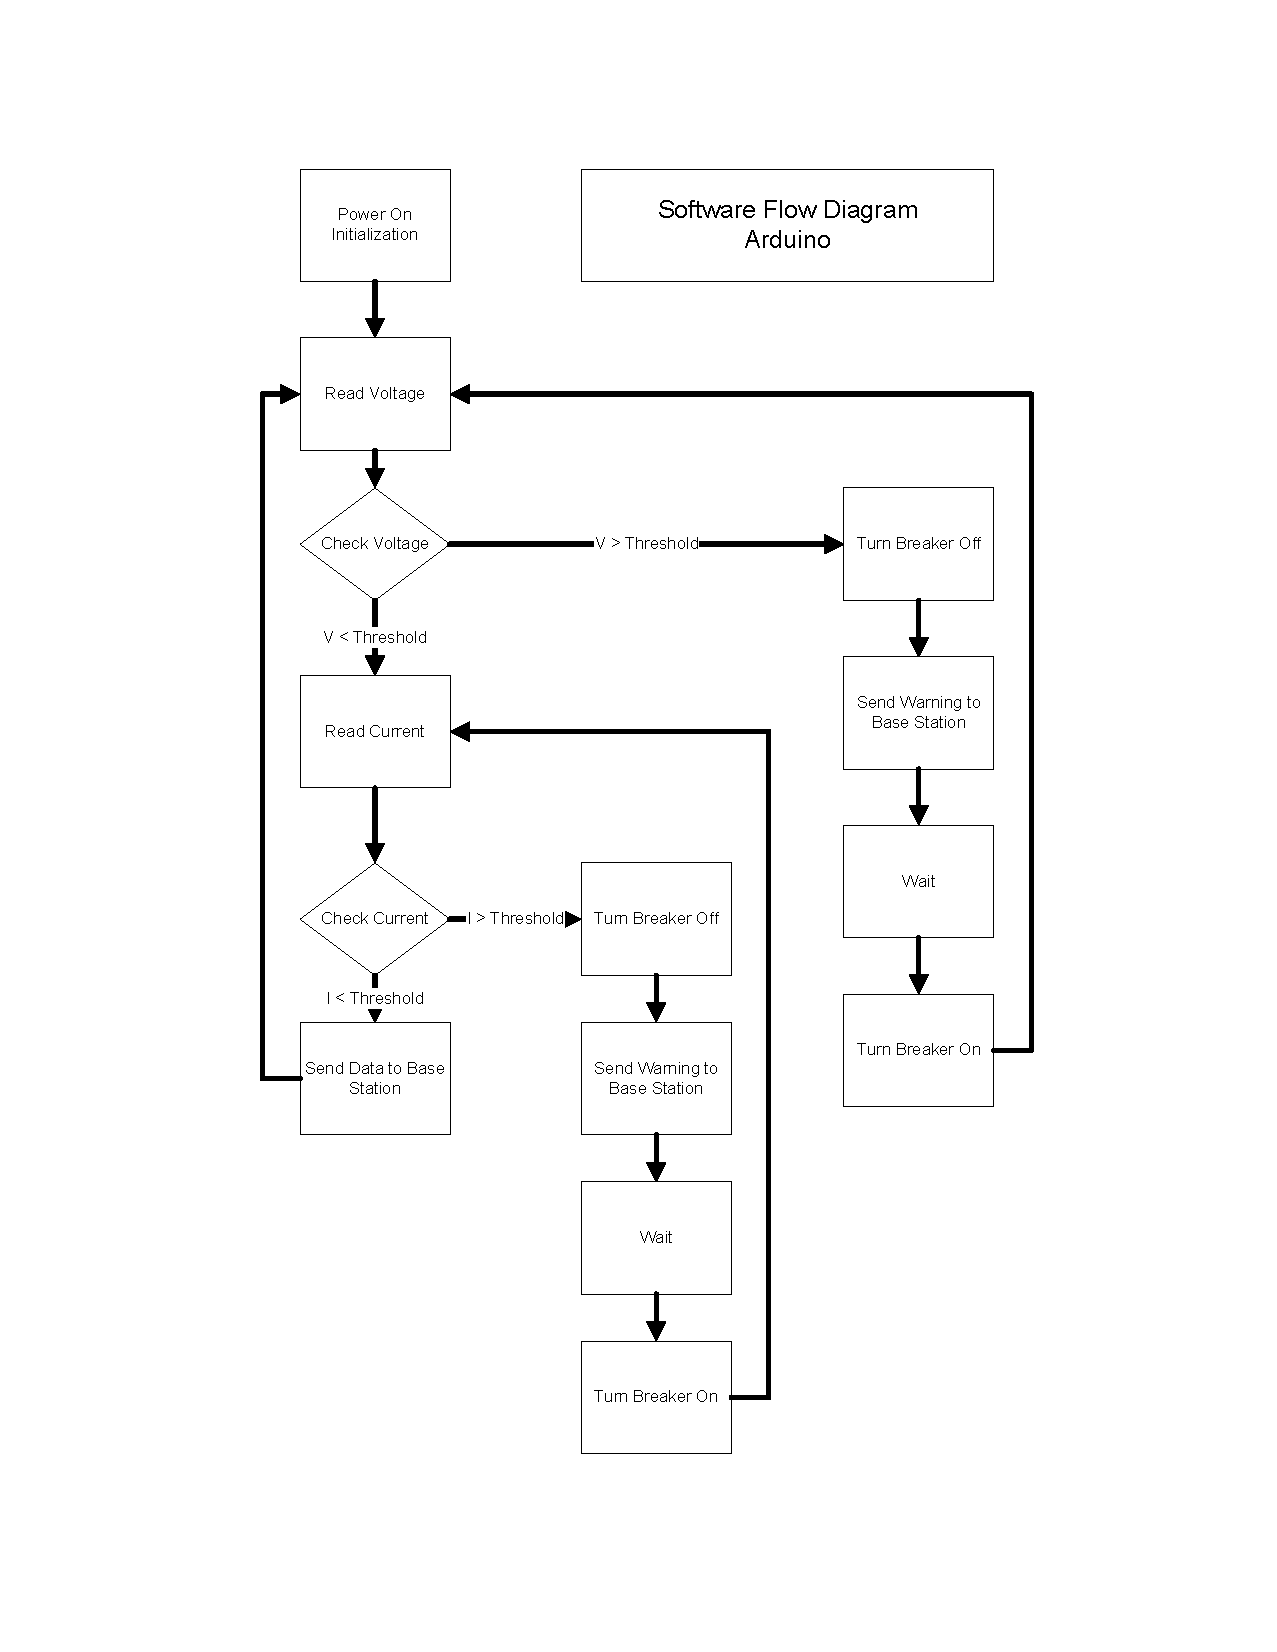
\includegraphics[height=2.5in]{includes/ArduinoSoftwareFlow}
	\caption{Arduino software flowchart.}
	\label{fig:arduino_software_flow}
	\end{center}
	\end{figure}
\end{frame}

\begin{frame}{Smart Breakers Software}
	\begin{block}{Software Design}
		\begin{itemize}
		\item <1-> Written using Arduino Sketchup IDE
		\item <2-> SPI interface to ADE7763 (SPI Arduino Library)
		\item <3-> Serial interface to Xbee radio (Xbee Arduino Library)
		\end{itemize}
	\end{block}
\end{frame}

% -- Amy's Power Supply
\section{Power Supply}
\begin{frame}{Power Supply}
	\begin{block}{Purpose}
		\begin{itemize}
		\item <1 -> Even though the PICA system monitors power it still needs to power itself
		\item <2 -> One generic supply for both subsystems
		\item <3 -> Switched mode power supply for efficiency
		\end{itemize}
	\end{block}
\end{frame}

\begin{frame}{Power Supply Hardware}
	\begin{figure}[htbp]
	\begin{center}
	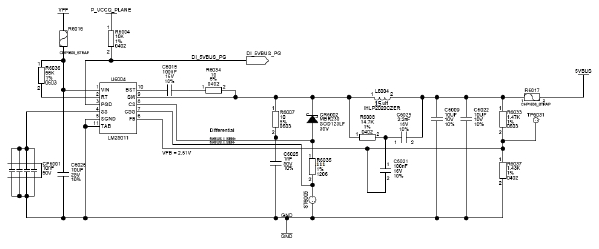
\includegraphics[width=4in]{includes/power_supply_schematic}
	\caption{Schematic for the PICA power supply.}
	\label{fig:ps_schematic}
	\end{center}
	\end{figure}
\end{frame}

\section{Project Finances}
\begin{frame}{Finances}
	\begin{block}{Project Finances}
		\begin{itemize}
		\item <1 -> Originally requested \$1000 from the Calvin Engineering Department
		\item <2 -> Granted \$700 for the project
		\item <3 -> To date our team has only spent approximately \$250
		\end{itemize}
	\end{block}
\end{frame}

\section{Questions}
\begin{frame}{Questions and Answers}
\begin{center}

\includegraphics[width=3in]{includes/cube_question}
\end{center}
\end{frame}
\end{document}
